\documentclass[twoside]{book}

% Packages required by doxygen
\usepackage{fixltx2e}
\usepackage{calc}
\usepackage{doxygen}
\usepackage[export]{adjustbox} % also loads graphicx
\usepackage{graphicx}
\usepackage[utf8]{inputenc}
\usepackage{makeidx}
\usepackage{multicol}
\usepackage{multirow}
\PassOptionsToPackage{warn}{textcomp}
\usepackage{textcomp}
\usepackage[nointegrals]{wasysym}
\usepackage[table]{xcolor}

% Font selection
\usepackage[T1]{fontenc}
\usepackage[scaled=.90]{helvet}
\usepackage{courier}
\usepackage{amssymb}
\usepackage{sectsty}
\renewcommand{\familydefault}{\sfdefault}
\allsectionsfont{%
  \fontseries{bc}\selectfont%
  \color{darkgray}%
}
\renewcommand{\DoxyLabelFont}{%
  \fontseries{bc}\selectfont%
  \color{darkgray}%
}
\newcommand{\+}{\discretionary{\mbox{\scriptsize$\hookleftarrow$}}{}{}}

% Page & text layout
\usepackage{geometry}
\geometry{%
  a4paper,%
  top=2.5cm,%
  bottom=2.5cm,%
  left=2.5cm,%
  right=2.5cm%
}
\tolerance=750
\hfuzz=15pt
\hbadness=750
\setlength{\emergencystretch}{15pt}
\setlength{\parindent}{0cm}
\setlength{\parskip}{3ex plus 2ex minus 2ex}
\makeatletter
\renewcommand{\paragraph}{%
  \@startsection{paragraph}{4}{0ex}{-1.0ex}{1.0ex}{%
    \normalfont\normalsize\bfseries\SS@parafont%
  }%
}
\renewcommand{\subparagraph}{%
  \@startsection{subparagraph}{5}{0ex}{-1.0ex}{1.0ex}{%
    \normalfont\normalsize\bfseries\SS@subparafont%
  }%
}
\makeatother

% Headers & footers
\usepackage{fancyhdr}
\pagestyle{fancyplain}
\fancyhead[LE]{\fancyplain{}{\bfseries\thepage}}
\fancyhead[CE]{\fancyplain{}{}}
\fancyhead[RE]{\fancyplain{}{\bfseries\leftmark}}
\fancyhead[LO]{\fancyplain{}{\bfseries\rightmark}}
\fancyhead[CO]{\fancyplain{}{}}
\fancyhead[RO]{\fancyplain{}{\bfseries\thepage}}
\fancyfoot[LE]{\fancyplain{}{}}
\fancyfoot[CE]{\fancyplain{}{}}
\fancyfoot[RE]{\fancyplain{}{\bfseries\scriptsize Generated by Doxygen }}
\fancyfoot[LO]{\fancyplain{}{\bfseries\scriptsize Generated by Doxygen }}
\fancyfoot[CO]{\fancyplain{}{}}
\fancyfoot[RO]{\fancyplain{}{}}
\renewcommand{\footrulewidth}{0.4pt}
\renewcommand{\chaptermark}[1]{%
  \markboth{#1}{}%
}
\renewcommand{\sectionmark}[1]{%
  \markright{\thesection\ #1}%
}

% Indices & bibliography
\usepackage{natbib}
\usepackage[titles]{tocloft}
\setcounter{tocdepth}{3}
\setcounter{secnumdepth}{5}
\makeindex

% Hyperlinks (required, but should be loaded last)
\usepackage{ifpdf}
\ifpdf
  \usepackage[pdftex,pagebackref=true]{hyperref}
\else
  \usepackage[ps2pdf,pagebackref=true]{hyperref}
\fi
\hypersetup{%
  colorlinks=true,%
  linkcolor=blue,%
  citecolor=blue,%
  unicode%
}

% Custom commands
\newcommand{\clearemptydoublepage}{%
  \newpage{\pagestyle{empty}\cleardoublepage}%
}

\usepackage{caption}
\captionsetup{labelsep=space,justification=centering,font={bf},singlelinecheck=off,skip=4pt,position=top}

%===== C O N T E N T S =====

\begin{document}

% Titlepage & ToC
\hypersetup{pageanchor=false,
             bookmarksnumbered=true,
             pdfencoding=unicode
            }
\pagenumbering{alph}
\begin{titlepage}
\vspace*{7cm}
\begin{center}%
{\Large Week 2 -\/ Shapes }\\
\vspace*{1cm}
{\large Generated by Doxygen 1.8.14}\\
\end{center}
\end{titlepage}
\clearemptydoublepage
\pagenumbering{roman}
\tableofcontents
\clearemptydoublepage
\pagenumbering{arabic}
\hypersetup{pageanchor=true}

%--- Begin generated contents ---
\chapter{Lab 2 -\/ Shapes}
\label{index}\hypertarget{index}{}This program gives you a basic S\+F\+ML winow in which to draw your shapes.

The classes and files you use are up to you. ~\newline
 This software froms the basis of your submission for lab book 1 
\chapter{Lab Book 1 Starter Code}
\label{md__r_e_a_d_m_e}
\Hypertarget{md__r_e_a_d_m_e}
Starter Code for lab book 1 -\/ Shapes

You will need to download the external libs from blackbaord. You can then clone this repo in the labsfolder. 
\chapter{Hierarchical Index}
\section{Class Hierarchy}
This inheritance list is sorted roughly, but not completely, alphabetically\+:\begin{DoxyCompactList}
\item Drawable\begin{DoxyCompactList}
\item \contentsline{section}{arc}{\pageref{classarc}}{}
\item \contentsline{section}{circle}{\pageref{classcircle}}{}
\item \contentsline{section}{dot}{\pageref{classdot}}{}
\item \contentsline{section}{ellipse}{\pageref{classellipse}}{}
\item \contentsline{section}{line}{\pageref{classline}}{}
\item \contentsline{section}{rectangle}{\pageref{classrectangle}}{}
\item \contentsline{section}{square}{\pageref{classsquare}}{}
\item \contentsline{section}{triangle}{\pageref{classtriangle}}{}
\end{DoxyCompactList}
\item \contentsline{section}{arc\+:\+:h}{\pageref{classarc_1_1h}}{}
\item \contentsline{section}{circle\+:\+:h}{\pageref{classcircle_1_1h}}{}
\end{DoxyCompactList}

\chapter{Class Index}
\section{Class List}
Here are the classes, structs, unions and interfaces with brief descriptions\+:\begin{DoxyCompactList}
\item\contentsline{section}{\mbox{\hyperlink{classarc}{arc}} }{\pageref{classarc}}{}
\item\contentsline{section}{\mbox{\hyperlink{classcircle}{circle}} }{\pageref{classcircle}}{}
\item\contentsline{section}{\mbox{\hyperlink{classdot}{dot}} }{\pageref{classdot}}{}
\item\contentsline{section}{\mbox{\hyperlink{classellipse}{ellipse}} }{\pageref{classellipse}}{}
\item\contentsline{section}{\mbox{\hyperlink{classarc_1_1h}{arc\+::h}} \\*Used to draw Arcs }{\pageref{classarc_1_1h}}{}
\item\contentsline{section}{\mbox{\hyperlink{classcircle_1_1h}{circle\+::h}} \\*Used to draw circle Shapes }{\pageref{classcircle_1_1h}}{}
\item\contentsline{section}{\mbox{\hyperlink{classline}{line}} }{\pageref{classline}}{}
\item\contentsline{section}{\mbox{\hyperlink{classrectangle}{rectangle}} }{\pageref{classrectangle}}{}
\item\contentsline{section}{\mbox{\hyperlink{classsquare}{square}} }{\pageref{classsquare}}{}
\item\contentsline{section}{\mbox{\hyperlink{classtriangle}{triangle}} }{\pageref{classtriangle}}{}
\end{DoxyCompactList}

\chapter{File Index}
\section{File List}
Here is a list of all documented files with brief descriptions\+:\begin{DoxyCompactList}
\item\contentsline{section}{include/{\bfseries arc.\+h} }{\pageref{arc_8h}}{}
\item\contentsline{section}{include/{\bfseries circle.\+h} }{\pageref{circle_8h}}{}
\item\contentsline{section}{include/\mbox{\hyperlink{dot_8h}{dot.\+h}} }{\pageref{dot_8h}}{}
\item\contentsline{section}{include/\mbox{\hyperlink{ellipse_8h}{ellipse.\+h}} }{\pageref{ellipse_8h}}{}
\item\contentsline{section}{include/\mbox{\hyperlink{line_8h}{line.\+h}} }{\pageref{line_8h}}{}
\item\contentsline{section}{include/{\bfseries main.\+h} }{\pageref{main_8h}}{}
\item\contentsline{section}{include/\mbox{\hyperlink{rectangle_8h}{rectangle.\+h}} }{\pageref{rectangle_8h}}{}
\item\contentsline{section}{include/\mbox{\hyperlink{square_8h}{square.\+h}} }{\pageref{square_8h}}{}
\item\contentsline{section}{include/\mbox{\hyperlink{triangle_8h}{triangle.\+h}} }{\pageref{triangle_8h}}{}
\item\contentsline{section}{src/\mbox{\hyperlink{arc_8cpp}{arc.\+cpp}} \\*Code used to draw Arcs }{\pageref{arc_8cpp}}{}
\item\contentsline{section}{src/\mbox{\hyperlink{main_8cpp}{main.\+cpp}} \\*Main file for the application }{\pageref{main_8cpp}}{}
\end{DoxyCompactList}

\chapter{Class Documentation}
\hypertarget{classarc}{}\section{arc Class Reference}
\label{classarc}\index{arc@{arc}}
Inheritance diagram for arc\+:\begin{figure}[H]
\begin{center}
\leavevmode
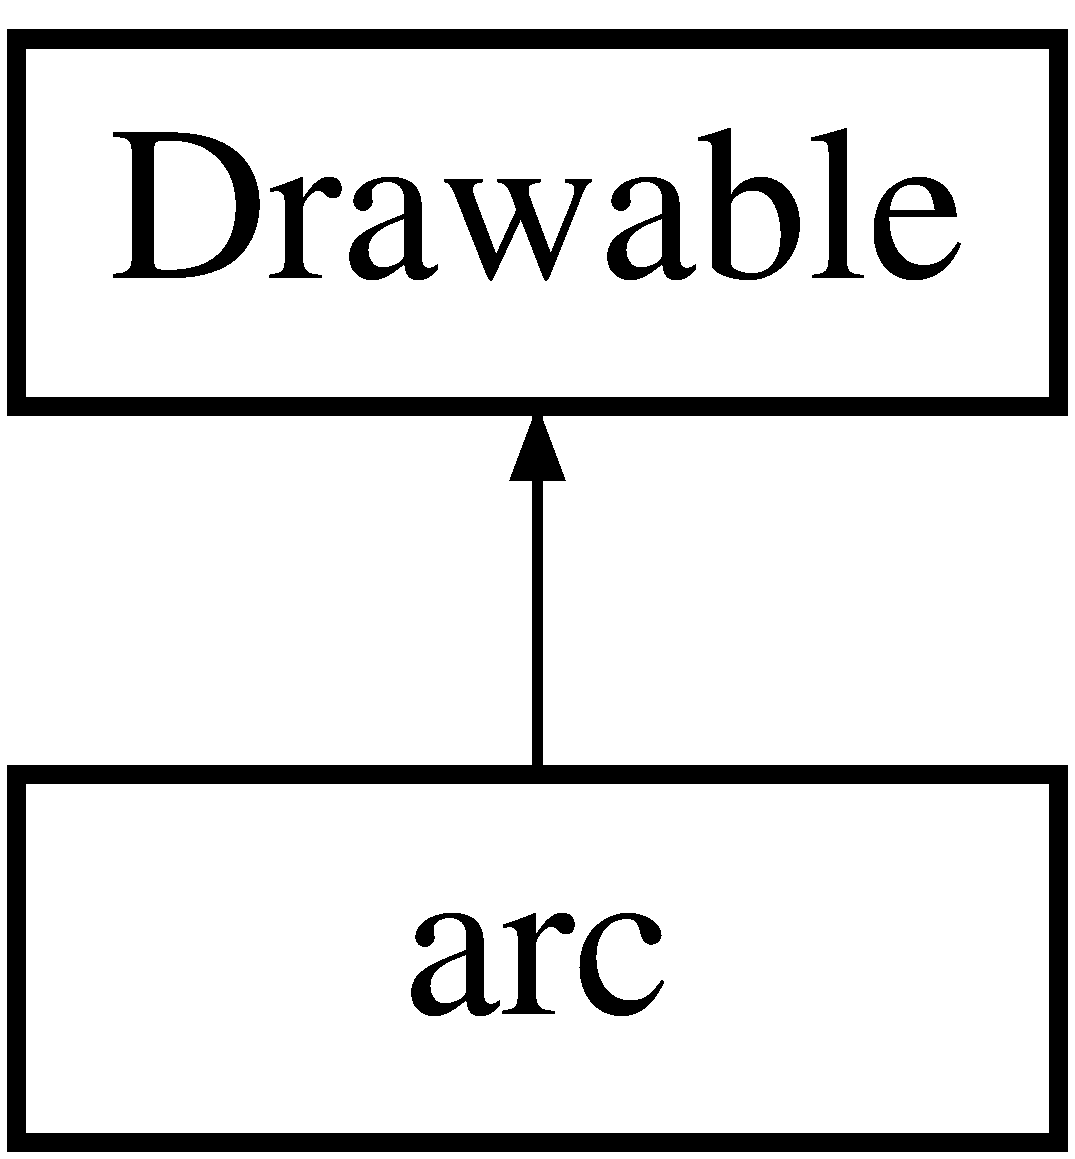
\includegraphics[height=2.000000cm]{classarc}
\end{center}
\end{figure}
\subsection*{Classes}
\begin{DoxyCompactItemize}
\item 
class \mbox{\hyperlink{classarc_1_1h}{h}}
\begin{DoxyCompactList}\small\item\em Used to draw Arcs. \end{DoxyCompactList}\end{DoxyCompactItemize}
\subsection*{Public Member Functions}
\begin{DoxyCompactItemize}
\item 
\mbox{\Hypertarget{classarc_af74708f0bbaf258e24ef12f713e3da72}\label{classarc_af74708f0bbaf258e24ef12f713e3da72}} 
void \mbox{\hyperlink{classarc_af74708f0bbaf258e24ef12f713e3da72}{calculate\+Vertices}} ()
\begin{DoxyCompactList}\small\item\em Calculates and sets the position and color of each Vertex. \end{DoxyCompactList}\item 
\mbox{\Hypertarget{classarc_aa90fc31672bae86b466e05d7107f9b31}\label{classarc_aa90fc31672bae86b466e05d7107f9b31}} 
\mbox{\hyperlink{classarc_aa90fc31672bae86b466e05d7107f9b31}{arc}} ()
\begin{DoxyCompactList}\small\item\em Constructs the object with default paramaters. \end{DoxyCompactList}\item 
\mbox{\hyperlink{classarc_a7904b57378159ca3de7005fd0a90a90a}{arc}} (float Xpos, float Y\+Pos, float X\+Radius, float Y\+Radius, float Start\+Theta, float End\+Theta, sf\+::\+Color New\+Color)
\begin{DoxyCompactList}\small\item\em Constructs the object with set paramaters. \end{DoxyCompactList}\item 
\mbox{\Hypertarget{classarc_a7ee6406fc154e5f92eba5ff140dd79af}\label{classarc_a7ee6406fc154e5f92eba5ff140dd79af}} 
\mbox{\hyperlink{classarc_a7ee6406fc154e5f92eba5ff140dd79af}{$\sim$arc}} ()
\begin{DoxyCompactList}\small\item\em Deconstructor. \end{DoxyCompactList}\item 
\mbox{\Hypertarget{classarc_aacf9c75f72272092f4a2241f4550f48b}\label{classarc_aacf9c75f72272092f4a2241f4550f48b}} 
void \mbox{\hyperlink{classarc_aacf9c75f72272092f4a2241f4550f48b}{draw}} (sf\+::\+Render\+Target \&target, sf\+::\+Render\+States states) const
\begin{DoxyCompactList}\small\item\em Draws the Object. \end{DoxyCompactList}\end{DoxyCompactItemize}


\subsection{Constructor \& Destructor Documentation}
\mbox{\Hypertarget{classarc_a7904b57378159ca3de7005fd0a90a90a}\label{classarc_a7904b57378159ca3de7005fd0a90a90a}} 
\index{arc@{arc}!arc@{arc}}
\index{arc@{arc}!arc@{arc}}
\subsubsection{\texorpdfstring{arc()}{arc()}}
{\footnotesize\ttfamily arc\+::arc (\begin{DoxyParamCaption}\item[{float}]{Xpos,  }\item[{float}]{Y\+Pos,  }\item[{float}]{Base,  }\item[{float}]{Height,  }\item[{float}]{Start\+Theta,  }\item[{float}]{End\+Theta,  }\item[{sf\+::\+Color}]{New\+Color }\end{DoxyParamCaption})}



Constructs the object with set paramaters. 


\begin{DoxyParams}{Parameters}
{\em Xpos} & X position. \\
\hline
{\em Ypos} & Y position. \\
\hline
{\em X\+Radius} & Radius on the X axis. \\
\hline
{\em Y\+Radius} & Radius on the Y axis. \\
\hline
{\em Start\+Theta} & Start Angle in Radians. \\
\hline
{\em End\+Theta} & End Angle in Radians. \\
\hline
{\em New\+Color} & Color of Shape. \\
\hline
\end{DoxyParams}


The documentation for this class was generated from the following files\+:\begin{DoxyCompactItemize}
\item 
include/arc.\+h\item 
src/\mbox{\hyperlink{arc_8cpp}{arc.\+cpp}}\end{DoxyCompactItemize}

\hypertarget{classcircle}{}\section{circle Class Reference}
\label{classcircle}\index{circle@{circle}}
Inheritance diagram for circle\+:\begin{figure}[H]
\begin{center}
\leavevmode
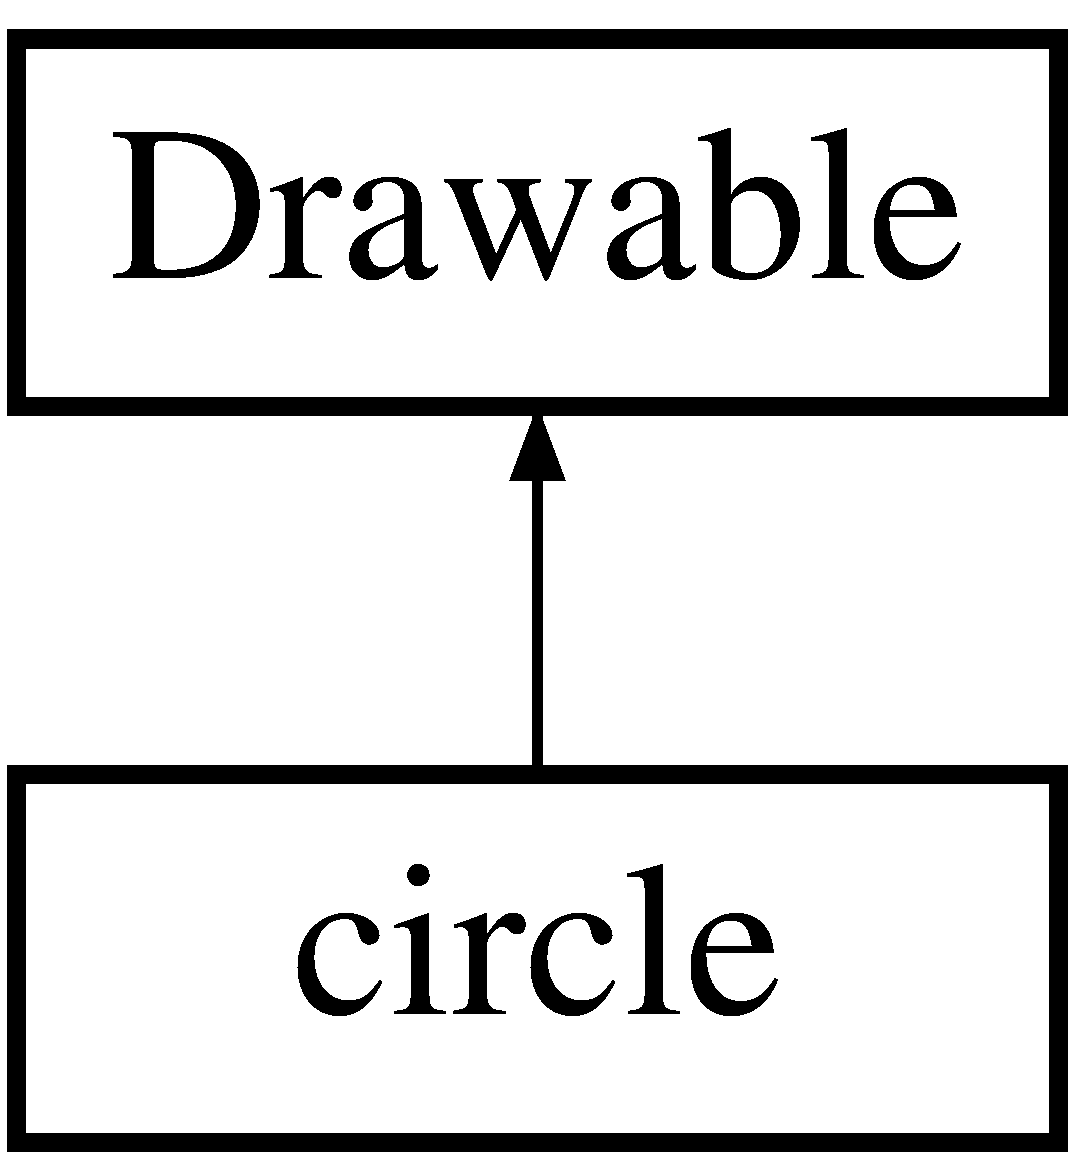
\includegraphics[height=2.000000cm]{classcircle}
\end{center}
\end{figure}
\subsection*{Classes}
\begin{DoxyCompactItemize}
\item 
class \mbox{\hyperlink{classcircle_1_1h}{h}}
\begin{DoxyCompactList}\small\item\em Used to draw circle Shapes. \end{DoxyCompactList}\end{DoxyCompactItemize}
\subsection*{Public Member Functions}
\begin{DoxyCompactItemize}
\item 
\mbox{\Hypertarget{classcircle_a59ddd77fe7255e30bd2d95d2e8114aec}\label{classcircle_a59ddd77fe7255e30bd2d95d2e8114aec}} 
void \mbox{\hyperlink{classcircle_a59ddd77fe7255e30bd2d95d2e8114aec}{calculate\+Vertices}} ()
\begin{DoxyCompactList}\small\item\em Calculates and sets the position and color of each Vertex. \end{DoxyCompactList}\item 
\mbox{\Hypertarget{classcircle_a4e0786fc75051f3bbe5de2e08ef9712d}\label{classcircle_a4e0786fc75051f3bbe5de2e08ef9712d}} 
\mbox{\hyperlink{classcircle_a4e0786fc75051f3bbe5de2e08ef9712d}{circle}} ()
\begin{DoxyCompactList}\small\item\em Constructs the object with default paramaters. \end{DoxyCompactList}\item 
\mbox{\hyperlink{classcircle_ad0b8c457c164f957281a8022308dace7}{circle}} (float Xpos, float Y\+Pos, float Radius, sf\+::\+Color New\+Color)
\begin{DoxyCompactList}\small\item\em Constructs the object with set paramaters. \end{DoxyCompactList}\item 
\mbox{\Hypertarget{classcircle_a6cc69d3a0c147bb2c7e2a4bd91490e75}\label{classcircle_a6cc69d3a0c147bb2c7e2a4bd91490e75}} 
void {\bfseries draw} (sf\+::\+Render\+Target \&target, sf\+::\+Render\+States states) const
\end{DoxyCompactItemize}


\subsection{Constructor \& Destructor Documentation}
\mbox{\Hypertarget{classcircle_ad0b8c457c164f957281a8022308dace7}\label{classcircle_ad0b8c457c164f957281a8022308dace7}} 
\index{circle@{circle}!circle@{circle}}
\index{circle@{circle}!circle@{circle}}
\subsubsection{\texorpdfstring{circle()}{circle()}}
{\footnotesize\ttfamily circle\+::circle (\begin{DoxyParamCaption}\item[{float}]{Xpos,  }\item[{float}]{Y\+Pos,  }\item[{float}]{Radius,  }\item[{sf\+::\+Color}]{New\+Color }\end{DoxyParamCaption})}



Constructs the object with set paramaters. 


\begin{DoxyParams}{Parameters}
{\em Xpos} & X position. \\
\hline
{\em Ypos} & Y position. \\
\hline
{\em Radius} & Radius of the circle. \\
\hline
{\em New\+Color} & Color of Shape. \\
\hline
\end{DoxyParams}


The documentation for this class was generated from the following files\+:\begin{DoxyCompactItemize}
\item 
include/circle.\+h\item 
src/circle.\+cpp\end{DoxyCompactItemize}

\hypertarget{classdot}{}\section{dot Class Reference}
\label{classdot}\index{dot@{dot}}
Inheritance diagram for dot\+:\begin{figure}[H]
\begin{center}
\leavevmode
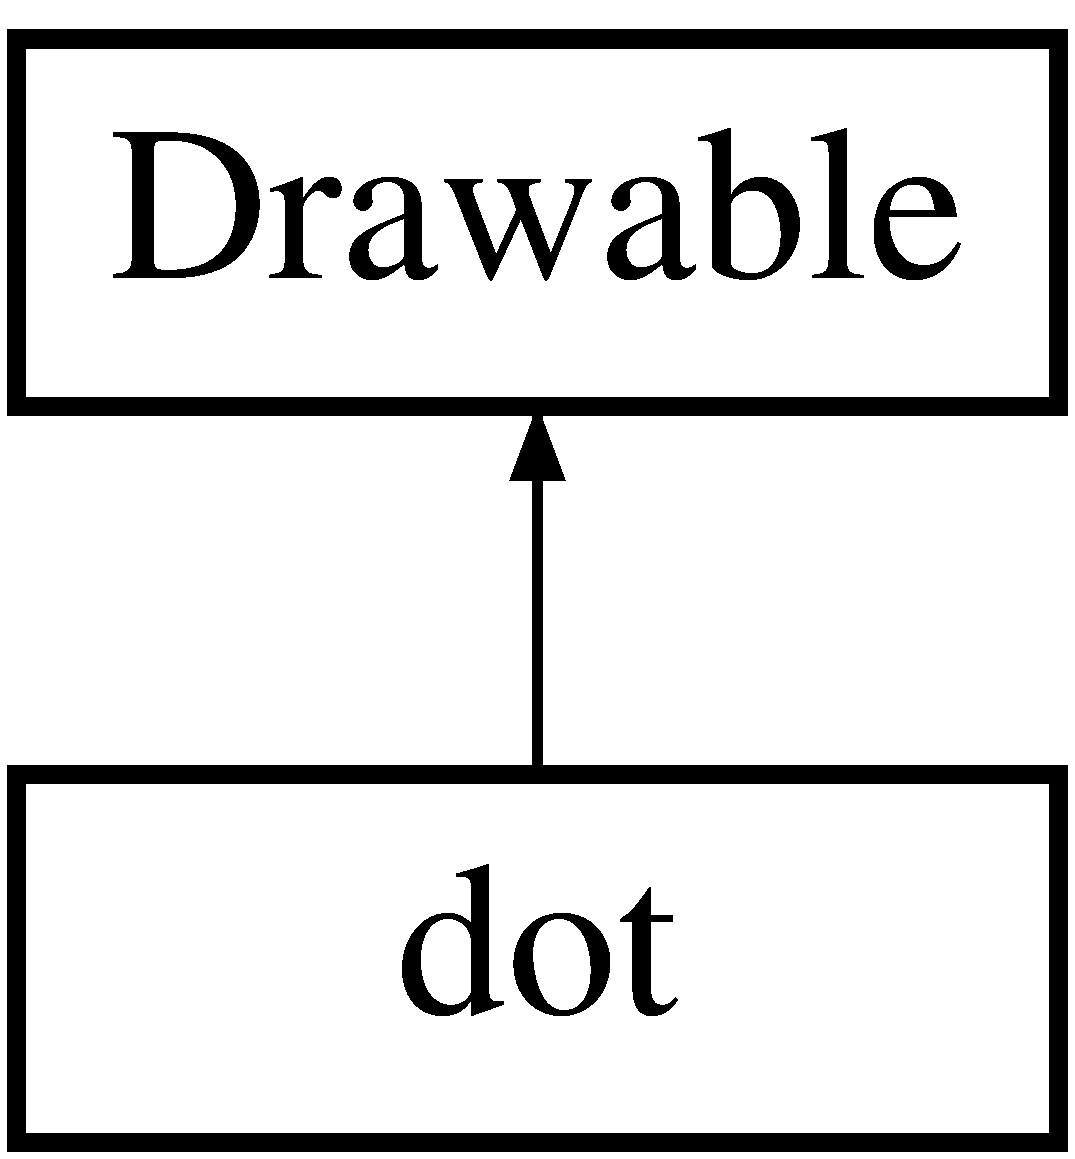
\includegraphics[height=2.000000cm]{classdot}
\end{center}
\end{figure}
\subsection*{Public Member Functions}
\begin{DoxyCompactItemize}
\item 
\mbox{\Hypertarget{classdot_ab7e7b07476ca33fb39c7eba358072dab}\label{classdot_ab7e7b07476ca33fb39c7eba358072dab}} 
void \mbox{\hyperlink{classdot_ab7e7b07476ca33fb39c7eba358072dab}{calculate\+Vertices}} ()
\begin{DoxyCompactList}\small\item\em Calculates and sets the position and color of each Vertex. \end{DoxyCompactList}\item 
\mbox{\Hypertarget{classdot_a8bb8093dfad084a2aba7dcd300cd7832}\label{classdot_a8bb8093dfad084a2aba7dcd300cd7832}} 
\mbox{\hyperlink{classdot_a8bb8093dfad084a2aba7dcd300cd7832}{dot}} ()
\begin{DoxyCompactList}\small\item\em Constructs the object with default paramaters. \end{DoxyCompactList}\item 
\mbox{\hyperlink{classdot_adafc58b4cfa749ca975280ed4367136e}{dot}} (float Xpos, float Y\+Pos, sf\+::\+Color New\+Color)
\begin{DoxyCompactList}\small\item\em Constructs the object with set paramaters. \end{DoxyCompactList}\item 
\mbox{\Hypertarget{classdot_a198816651106b5ad7e853d8fcda1223d}\label{classdot_a198816651106b5ad7e853d8fcda1223d}} 
void {\bfseries draw} (sf\+::\+Render\+Target \&target, sf\+::\+Render\+States states) const
\end{DoxyCompactItemize}


\subsection{Constructor \& Destructor Documentation}
\mbox{\Hypertarget{classdot_adafc58b4cfa749ca975280ed4367136e}\label{classdot_adafc58b4cfa749ca975280ed4367136e}} 
\index{dot@{dot}!dot@{dot}}
\index{dot@{dot}!dot@{dot}}
\subsubsection{\texorpdfstring{dot()}{dot()}}
{\footnotesize\ttfamily dot\+::dot (\begin{DoxyParamCaption}\item[{float}]{Xpos,  }\item[{float}]{Y\+Pos,  }\item[{sf\+::\+Color}]{New\+Color }\end{DoxyParamCaption})}



Constructs the object with set paramaters. 


\begin{DoxyParams}{Parameters}
{\em Xpos} & X position. \\
\hline
{\em Ypos} & Y position. \\
\hline
{\em New\+Color} & Color. \\
\hline
\end{DoxyParams}


The documentation for this class was generated from the following files\+:\begin{DoxyCompactItemize}
\item 
include/\mbox{\hyperlink{dot_8h}{dot.\+h}}\item 
src/dot.\+cpp\end{DoxyCompactItemize}

\hypertarget{classellipse}{}\section{ellipse Class Reference}
\label{classellipse}\index{ellipse@{ellipse}}
Inheritance diagram for ellipse\+:\begin{figure}[H]
\begin{center}
\leavevmode
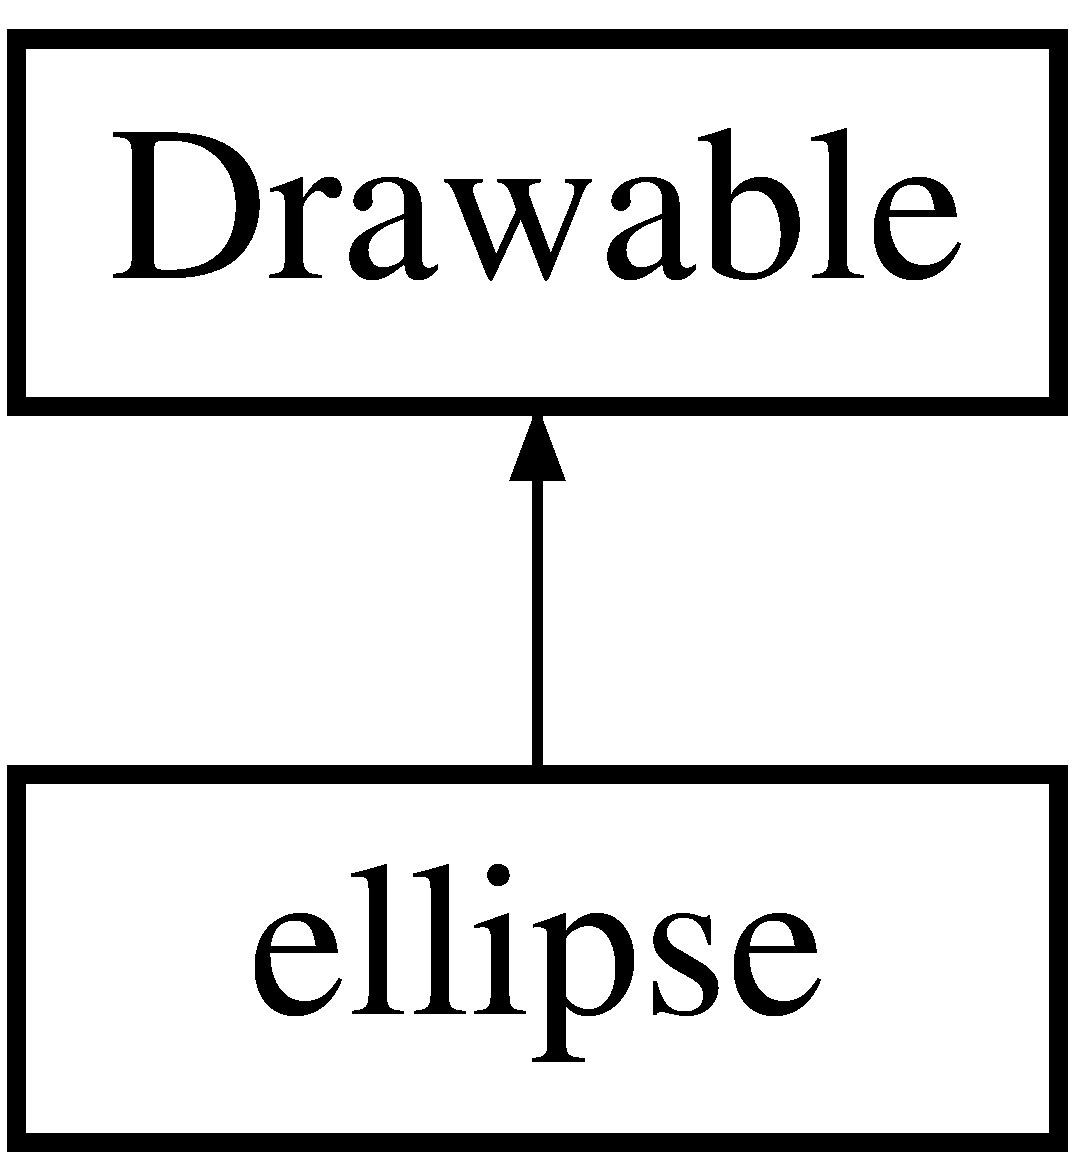
\includegraphics[height=2.000000cm]{classellipse}
\end{center}
\end{figure}
\subsection*{Public Member Functions}
\begin{DoxyCompactItemize}
\item 
\mbox{\Hypertarget{classellipse_a59c2f682625538eb3f5ec106d9755f8f}\label{classellipse_a59c2f682625538eb3f5ec106d9755f8f}} 
void \mbox{\hyperlink{classellipse_a59c2f682625538eb3f5ec106d9755f8f}{calculate\+Vertices}} ()
\begin{DoxyCompactList}\small\item\em Calculates and sets the position and color of each Vertex. \end{DoxyCompactList}\item 
\mbox{\Hypertarget{classellipse_a4176fad8b9a976e08817c56cbefdffc7}\label{classellipse_a4176fad8b9a976e08817c56cbefdffc7}} 
\mbox{\hyperlink{classellipse_a4176fad8b9a976e08817c56cbefdffc7}{ellipse}} ()
\begin{DoxyCompactList}\small\item\em Constructs the object with default paramaters. \end{DoxyCompactList}\item 
\mbox{\hyperlink{classellipse_a7eabcab8be3f231227197c61b3f86af7}{ellipse}} (float Xpos, float Y\+Pos, float X\+Radius, float Y\+Radius, sf\+::\+Color New\+Color)
\begin{DoxyCompactList}\small\item\em Constructs the object with set paramaters. \end{DoxyCompactList}\item 
\mbox{\Hypertarget{classellipse_ad28e53a614a981a5937edb65a05e4e38}\label{classellipse_ad28e53a614a981a5937edb65a05e4e38}} 
void {\bfseries draw} (sf\+::\+Render\+Target \&target, sf\+::\+Render\+States states) const
\end{DoxyCompactItemize}


\subsection{Constructor \& Destructor Documentation}
\mbox{\Hypertarget{classellipse_a7eabcab8be3f231227197c61b3f86af7}\label{classellipse_a7eabcab8be3f231227197c61b3f86af7}} 
\index{ellipse@{ellipse}!ellipse@{ellipse}}
\index{ellipse@{ellipse}!ellipse@{ellipse}}
\subsubsection{\texorpdfstring{ellipse()}{ellipse()}}
{\footnotesize\ttfamily ellipse\+::ellipse (\begin{DoxyParamCaption}\item[{float}]{Xpos,  }\item[{float}]{Y\+Pos,  }\item[{float}]{X\+Radius,  }\item[{float}]{Y\+Radius,  }\item[{sf\+::\+Color}]{New\+Color }\end{DoxyParamCaption})}



Constructs the object with set paramaters. 


\begin{DoxyParams}{Parameters}
{\em Xpos} & X position. \\
\hline
{\em Ypos} & Y position. \\
\hline
{\em X\+Radius} & Radius on the X axis. \\
\hline
{\em Y\+Radius} & Radius on the Y axis. \\
\hline
{\em New\+Color} & Color of Shape. \\
\hline
\end{DoxyParams}


The documentation for this class was generated from the following files\+:\begin{DoxyCompactItemize}
\item 
include/\mbox{\hyperlink{ellipse_8h}{ellipse.\+h}}\item 
src/ellipse.\+cpp\end{DoxyCompactItemize}

\hypertarget{classarc_1_1h}{}\section{arc\+:\+:h Class Reference}
\label{classarc_1_1h}\index{arc\+::h@{arc\+::h}}


Used to draw Arcs.  




{\ttfamily \#include $<$arc.\+h$>$}



\subsection{Detailed Description}
Used to draw Arcs. 

The documentation for this class was generated from the following file\+:\begin{DoxyCompactItemize}
\item 
include/arc.\+h\end{DoxyCompactItemize}

\hypertarget{classcircle_1_1h}{}\section{circle\+:\+:h Class Reference}
\label{classcircle_1_1h}\index{circle\+::h@{circle\+::h}}


Used to draw circle Shapes.  




{\ttfamily \#include $<$circle.\+h$>$}



\subsection{Detailed Description}
Used to draw circle Shapes. 

The documentation for this class was generated from the following file\+:\begin{DoxyCompactItemize}
\item 
include/circle.\+h\end{DoxyCompactItemize}

\hypertarget{classline}{}\section{line Class Reference}
\label{classline}\index{line@{line}}
Inheritance diagram for line\+:\begin{figure}[H]
\begin{center}
\leavevmode
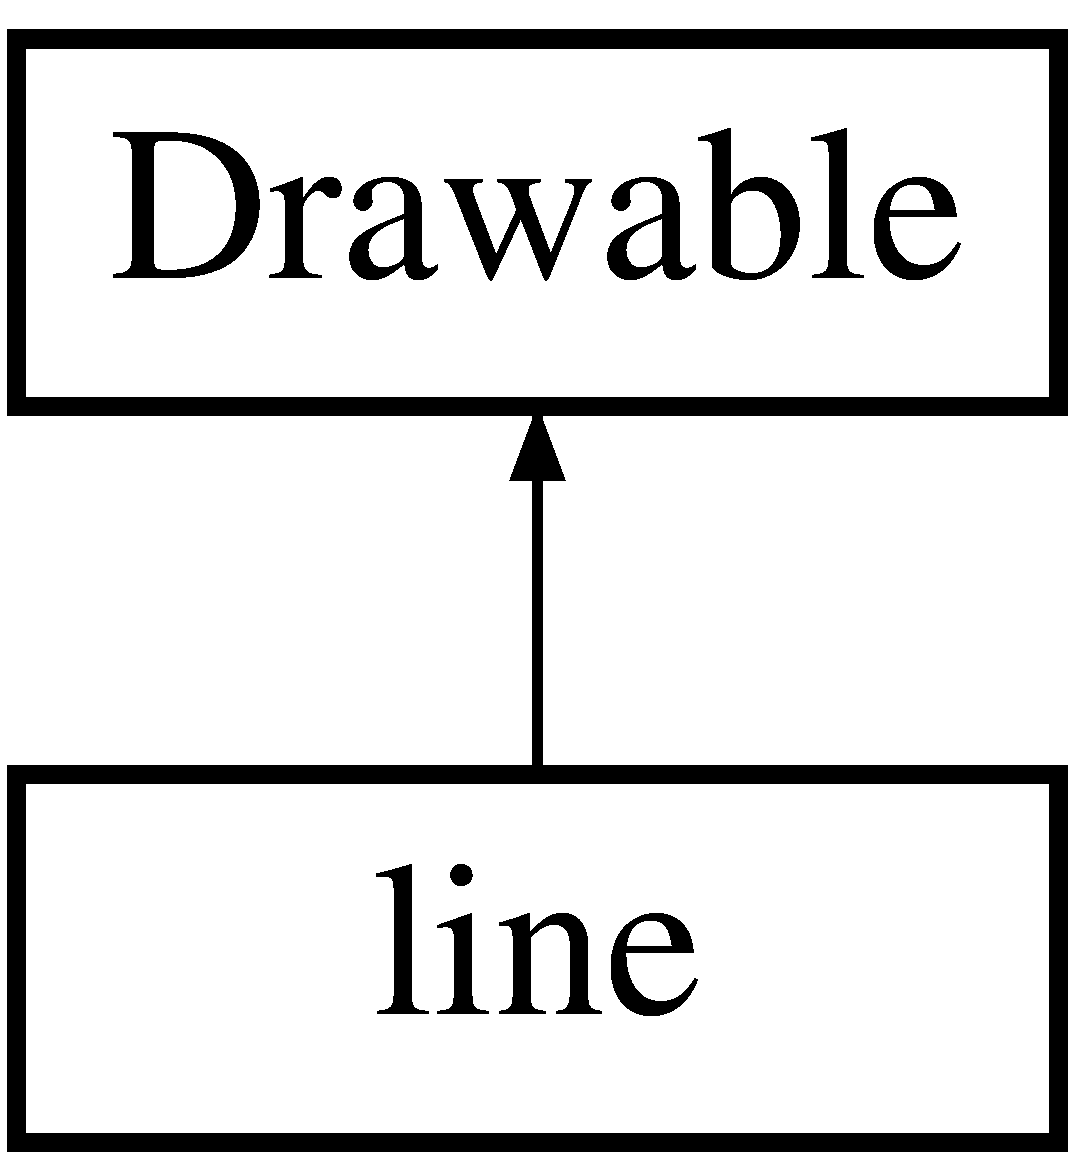
\includegraphics[height=2.000000cm]{classline}
\end{center}
\end{figure}
\subsection*{Public Member Functions}
\begin{DoxyCompactItemize}
\item 
\mbox{\Hypertarget{classline_a0b04699a018fa489119b3f7b98ecad60}\label{classline_a0b04699a018fa489119b3f7b98ecad60}} 
void \mbox{\hyperlink{classline_a0b04699a018fa489119b3f7b98ecad60}{calculate\+Vertices}} ()
\begin{DoxyCompactList}\small\item\em Calculates and sets the position and color of each Vertex. \end{DoxyCompactList}\item 
\mbox{\Hypertarget{classline_a854d4e37d6dc6af1c7cd08cb801c6c26}\label{classline_a854d4e37d6dc6af1c7cd08cb801c6c26}} 
\mbox{\hyperlink{classline_a854d4e37d6dc6af1c7cd08cb801c6c26}{line}} ()
\begin{DoxyCompactList}\small\item\em Constructs the object with default paramaters. \end{DoxyCompactList}\item 
\mbox{\hyperlink{classline_a86e47bbc81b214314dd46e20e4bd2d8b}{line}} (float XposA, float Y\+PosA, float X\+PosB, float Y\+PosB, sf\+::\+Color New\+Color)
\begin{DoxyCompactList}\small\item\em Constructs the object with set paramaters. \end{DoxyCompactList}\item 
\mbox{\Hypertarget{classline_ad439ea0b0f3df62fc3dc4a3a65c1ed9a}\label{classline_ad439ea0b0f3df62fc3dc4a3a65c1ed9a}} 
void {\bfseries draw} (sf\+::\+Render\+Target \&target, sf\+::\+Render\+States states) const
\end{DoxyCompactItemize}


\subsection{Constructor \& Destructor Documentation}
\mbox{\Hypertarget{classline_a86e47bbc81b214314dd46e20e4bd2d8b}\label{classline_a86e47bbc81b214314dd46e20e4bd2d8b}} 
\index{line@{line}!line@{line}}
\index{line@{line}!line@{line}}
\subsubsection{\texorpdfstring{line()}{line()}}
{\footnotesize\ttfamily line\+::line (\begin{DoxyParamCaption}\item[{float}]{XposA,  }\item[{float}]{Y\+PosA,  }\item[{float}]{X\+PosB,  }\item[{float}]{Y\+PosB,  }\item[{sf\+::\+Color}]{New\+Color }\end{DoxyParamCaption})}



Constructs the object with set paramaters. 


\begin{DoxyParams}{Parameters}
{\em XposA} & X position of point A. \\
\hline
{\em YposA} & Y position of point A. \\
\hline
{\em XposB} & X position of point B. \\
\hline
{\em YposB} & Y position of point B. \\
\hline
{\em New\+Color} & Color of Shape. \\
\hline
\end{DoxyParams}


The documentation for this class was generated from the following files\+:\begin{DoxyCompactItemize}
\item 
include/\mbox{\hyperlink{line_8h}{line.\+h}}\item 
src/line.\+cpp\end{DoxyCompactItemize}

\hypertarget{classrectangle}{}\section{rectangle Class Reference}
\label{classrectangle}\index{rectangle@{rectangle}}
Inheritance diagram for rectangle\+:\begin{figure}[H]
\begin{center}
\leavevmode
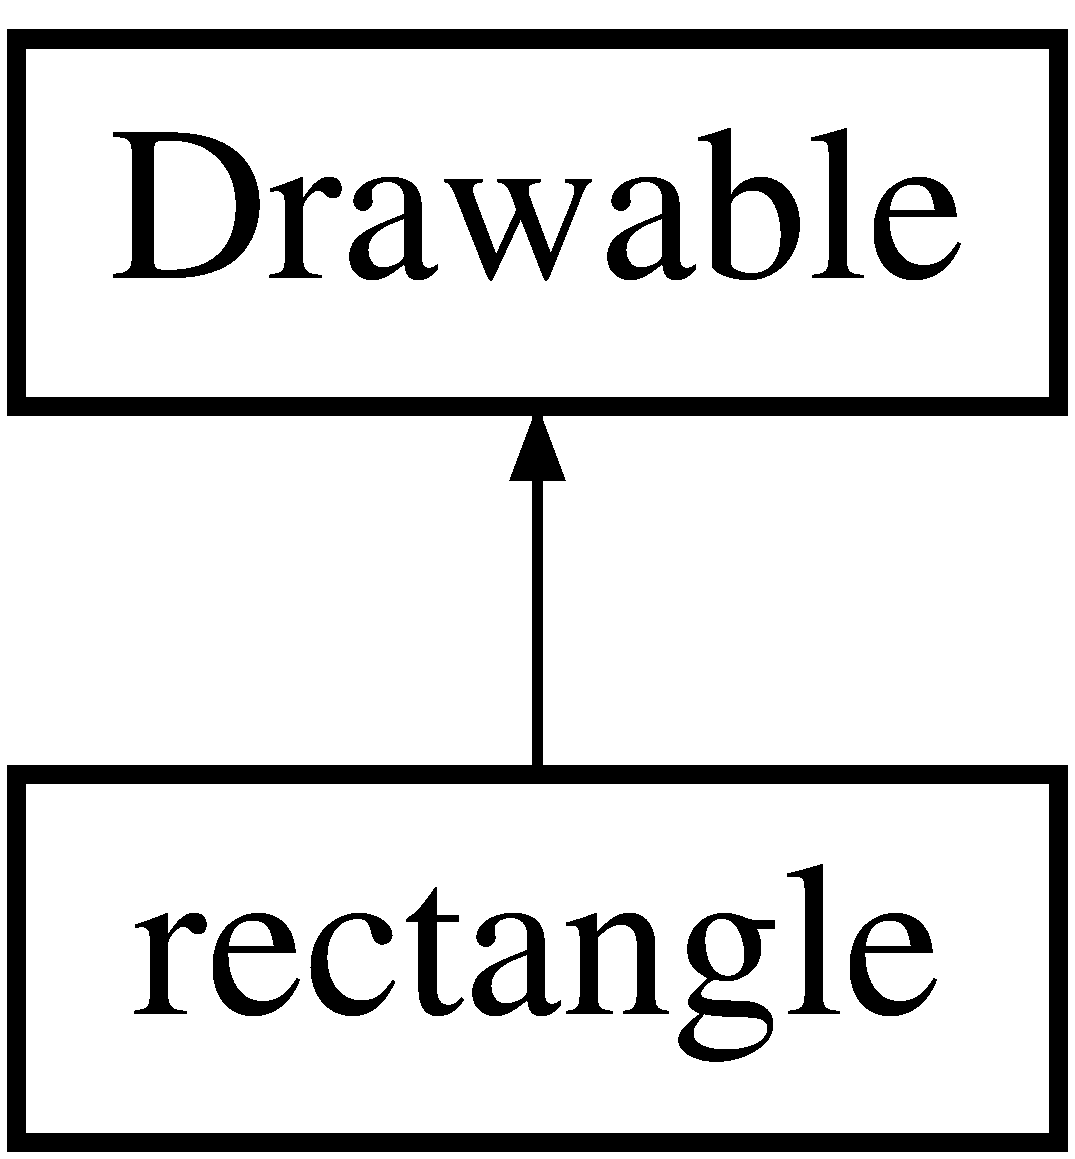
\includegraphics[height=2.000000cm]{classrectangle}
\end{center}
\end{figure}
\subsection*{Public Member Functions}
\begin{DoxyCompactItemize}
\item 
\mbox{\Hypertarget{classrectangle_a8f448e02e2ffcde7cde242d1486b3ede}\label{classrectangle_a8f448e02e2ffcde7cde242d1486b3ede}} 
void \mbox{\hyperlink{classrectangle_a8f448e02e2ffcde7cde242d1486b3ede}{calculate\+Vertices}} ()
\begin{DoxyCompactList}\small\item\em Calculates and sets the position and color of each Vertex. \end{DoxyCompactList}\item 
\mbox{\Hypertarget{classrectangle_acdc53c26d992570f77862a76aa6c07e7}\label{classrectangle_acdc53c26d992570f77862a76aa6c07e7}} 
\mbox{\hyperlink{classrectangle_acdc53c26d992570f77862a76aa6c07e7}{rectangle}} ()
\begin{DoxyCompactList}\small\item\em Constructs the object with default paramaters. \end{DoxyCompactList}\item 
\mbox{\hyperlink{classrectangle_add36bb7ea2c626fbc9f4e3534567e6b6}{rectangle}} (float Xpos, float Y\+Pos, float Base, float Height, sf\+::\+Color New\+Color)
\begin{DoxyCompactList}\small\item\em Constructs the object with set paramaters. \end{DoxyCompactList}\item 
\mbox{\Hypertarget{classrectangle_a96d85bad6c91f6188f3752731f4c1aaa}\label{classrectangle_a96d85bad6c91f6188f3752731f4c1aaa}} 
void {\bfseries draw} (sf\+::\+Render\+Target \&target, sf\+::\+Render\+States states) const
\end{DoxyCompactItemize}


\subsection{Constructor \& Destructor Documentation}
\mbox{\Hypertarget{classrectangle_add36bb7ea2c626fbc9f4e3534567e6b6}\label{classrectangle_add36bb7ea2c626fbc9f4e3534567e6b6}} 
\index{rectangle@{rectangle}!rectangle@{rectangle}}
\index{rectangle@{rectangle}!rectangle@{rectangle}}
\subsubsection{\texorpdfstring{rectangle()}{rectangle()}}
{\footnotesize\ttfamily rectangle\+::rectangle (\begin{DoxyParamCaption}\item[{float}]{Xpos,  }\item[{float}]{Y\+Pos,  }\item[{float}]{Base,  }\item[{float}]{Height,  }\item[{sf\+::\+Color}]{New\+Color }\end{DoxyParamCaption})}



Constructs the object with set paramaters. 


\begin{DoxyParams}{Parameters}
{\em Xpos} & X position. \\
\hline
{\em Ypos} & Y position. \\
\hline
{\em Base} & length of the base of the object. \\
\hline
{\em Height} & height of the object. \\
\hline
{\em New\+Color} & Color of Shape. \\
\hline
\end{DoxyParams}


The documentation for this class was generated from the following files\+:\begin{DoxyCompactItemize}
\item 
include/\mbox{\hyperlink{rectangle_8h}{rectangle.\+h}}\item 
src/rectangle.\+cpp\end{DoxyCompactItemize}

\hypertarget{classsquare}{}\section{square Class Reference}
\label{classsquare}\index{square@{square}}
Inheritance diagram for square\+:\begin{figure}[H]
\begin{center}
\leavevmode
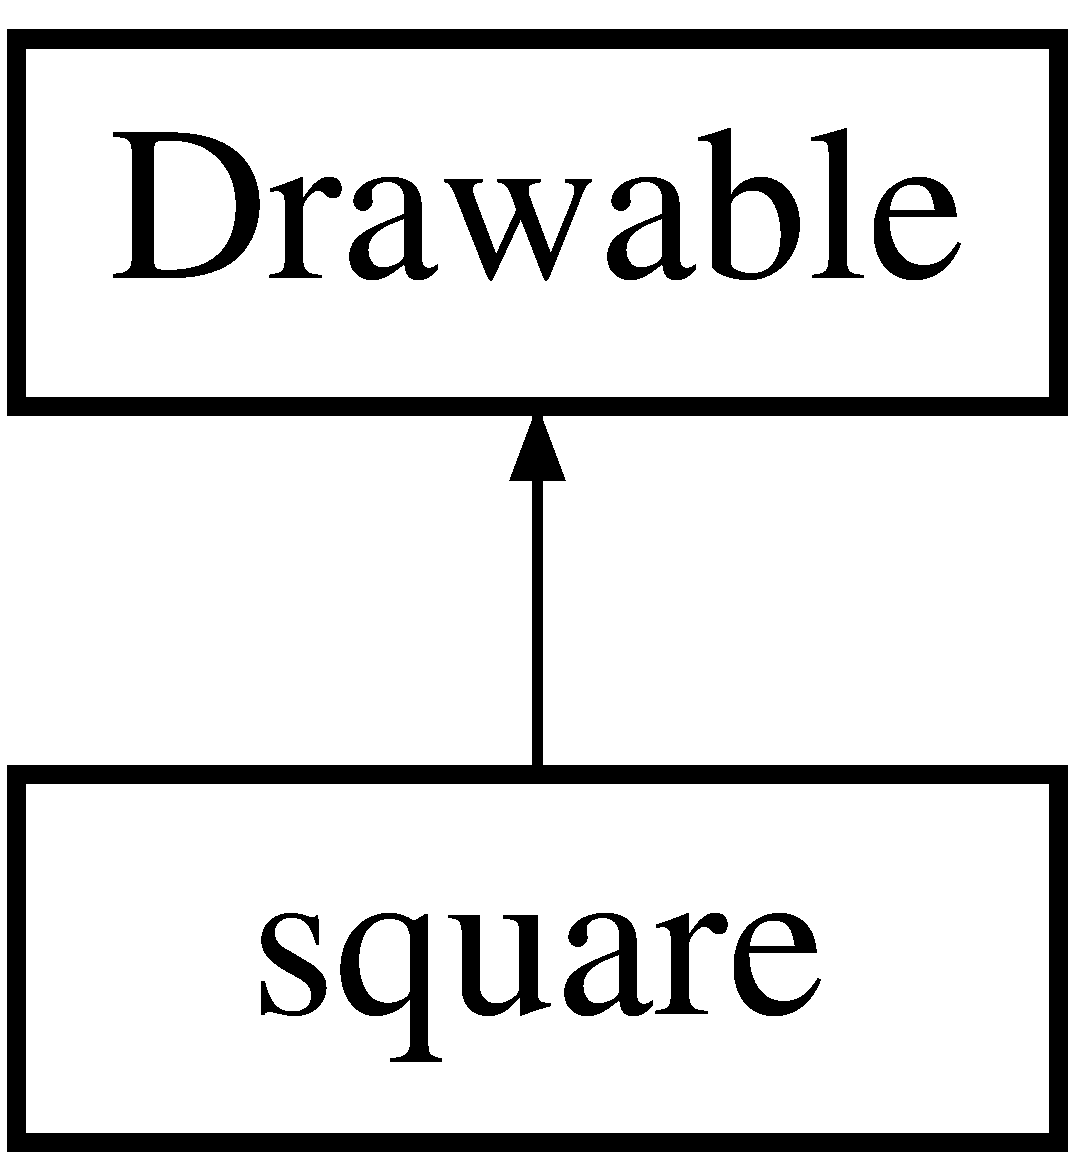
\includegraphics[height=2.000000cm]{classsquare}
\end{center}
\end{figure}
\subsection*{Public Member Functions}
\begin{DoxyCompactItemize}
\item 
\mbox{\Hypertarget{classsquare_a1d4d65c833348a55ad24eddaa8bcd098}\label{classsquare_a1d4d65c833348a55ad24eddaa8bcd098}} 
void \mbox{\hyperlink{classsquare_a1d4d65c833348a55ad24eddaa8bcd098}{calculate\+Vertices}} ()
\begin{DoxyCompactList}\small\item\em Calculates and sets the position and color of each Vertex. \end{DoxyCompactList}\item 
\mbox{\Hypertarget{classsquare_ab244ecd9e1c5f467c2fa889d25d01766}\label{classsquare_ab244ecd9e1c5f467c2fa889d25d01766}} 
\mbox{\hyperlink{classsquare_ab244ecd9e1c5f467c2fa889d25d01766}{square}} ()
\begin{DoxyCompactList}\small\item\em Constructs the object with default paramaters. \end{DoxyCompactList}\item 
\mbox{\hyperlink{classsquare_acd85b37d46decbe33655616837fd3972}{square}} (float Xpos, float Y\+Pos, float Length, sf\+::\+Color New\+Color)
\begin{DoxyCompactList}\small\item\em Constructs the object with set paramaters. \end{DoxyCompactList}\item 
\mbox{\Hypertarget{classsquare_a40bed2f326f5bf227e8efec61454eb4d}\label{classsquare_a40bed2f326f5bf227e8efec61454eb4d}} 
void {\bfseries draw} (sf\+::\+Render\+Target \&target, sf\+::\+Render\+States states) const
\end{DoxyCompactItemize}


\subsection{Constructor \& Destructor Documentation}
\mbox{\Hypertarget{classsquare_acd85b37d46decbe33655616837fd3972}\label{classsquare_acd85b37d46decbe33655616837fd3972}} 
\index{square@{square}!square@{square}}
\index{square@{square}!square@{square}}
\subsubsection{\texorpdfstring{square()}{square()}}
{\footnotesize\ttfamily square\+::square (\begin{DoxyParamCaption}\item[{float}]{Xpos,  }\item[{float}]{Y\+Pos,  }\item[{float}]{Length,  }\item[{sf\+::\+Color}]{New\+Color }\end{DoxyParamCaption})}



Constructs the object with set paramaters. 


\begin{DoxyParams}{Parameters}
{\em Xpos} & X position. \\
\hline
{\em Ypos} & Y position. \\
\hline
{\em Lenght} & size of the Square. \\
\hline
{\em New\+Color} & Color of Shape. \\
\hline
\end{DoxyParams}


The documentation for this class was generated from the following files\+:\begin{DoxyCompactItemize}
\item 
include/\mbox{\hyperlink{square_8h}{square.\+h}}\item 
src/square.\+cpp\end{DoxyCompactItemize}

\hypertarget{classtriangle}{}\section{triangle Class Reference}
\label{classtriangle}\index{triangle@{triangle}}
Inheritance diagram for triangle\+:\begin{figure}[H]
\begin{center}
\leavevmode
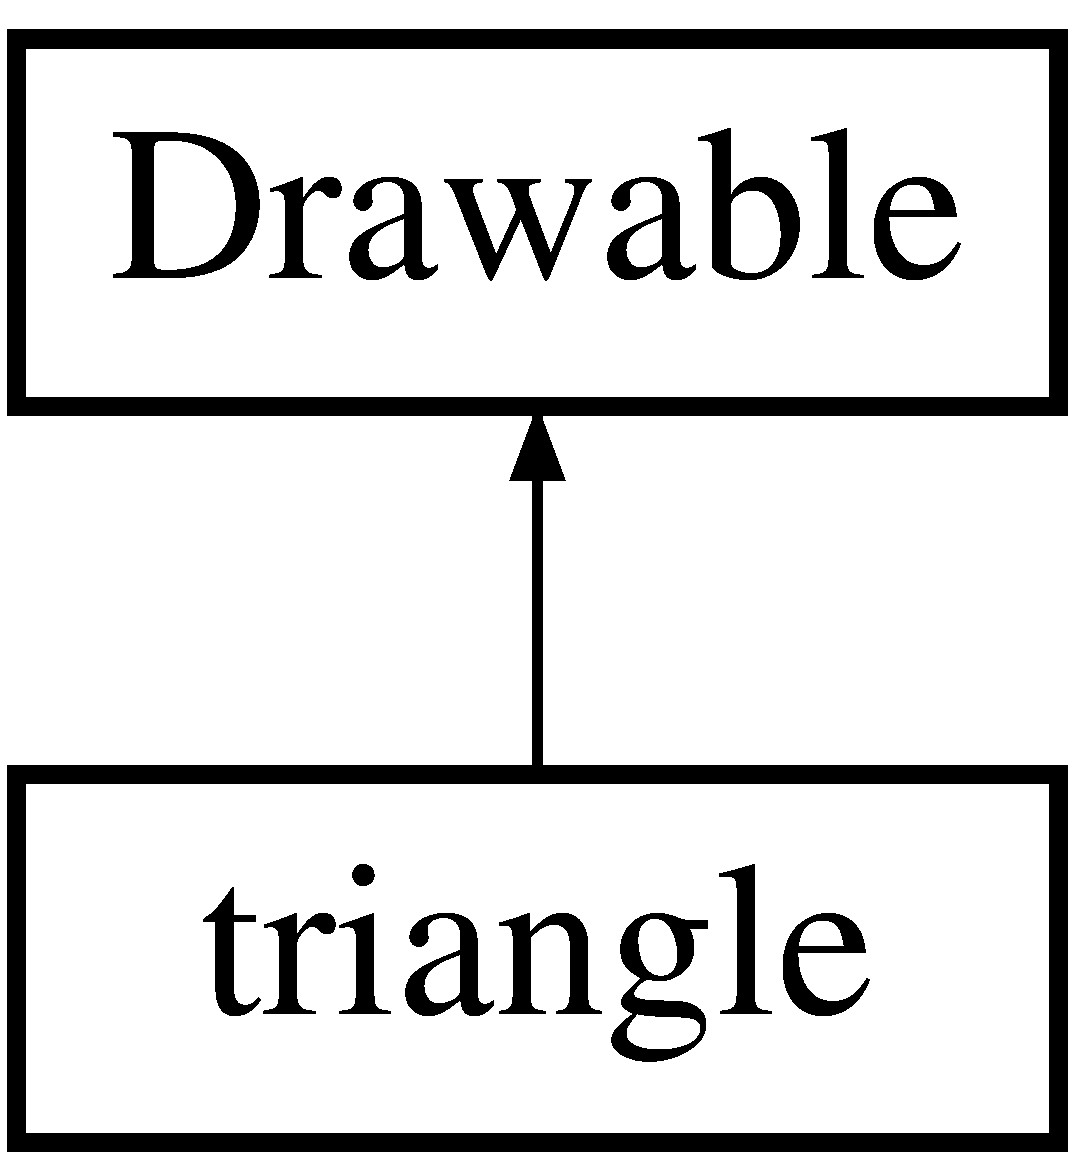
\includegraphics[height=2.000000cm]{classtriangle}
\end{center}
\end{figure}
\subsection*{Public Member Functions}
\begin{DoxyCompactItemize}
\item 
\mbox{\Hypertarget{classtriangle_a9a589314e2633a305644f5ac3a317d56}\label{classtriangle_a9a589314e2633a305644f5ac3a317d56}} 
void \mbox{\hyperlink{classtriangle_a9a589314e2633a305644f5ac3a317d56}{calculate\+Vertices}} ()
\begin{DoxyCompactList}\small\item\em Calculates and sets the position and color of each Vertex. \end{DoxyCompactList}\item 
\mbox{\Hypertarget{classtriangle_ac176bae9dc8cd99ca393c9f360760387}\label{classtriangle_ac176bae9dc8cd99ca393c9f360760387}} 
\mbox{\hyperlink{classtriangle_ac176bae9dc8cd99ca393c9f360760387}{triangle}} ()
\begin{DoxyCompactList}\small\item\em Constructs the object with default paramaters. \end{DoxyCompactList}\item 
\mbox{\hyperlink{classtriangle_aa856188746c2435f53441025d4181c51}{triangle}} (float Xpos, float Y\+Pos, float Base, float Height, sf\+::\+Color New\+Color)
\begin{DoxyCompactList}\small\item\em Constructs the object with set paramaters. \end{DoxyCompactList}\item 
\mbox{\Hypertarget{classtriangle_a9c2634977859ba059a89bce5323e8037}\label{classtriangle_a9c2634977859ba059a89bce5323e8037}} 
void {\bfseries draw} (sf\+::\+Render\+Target \&target, sf\+::\+Render\+States states) const
\end{DoxyCompactItemize}


\subsection{Constructor \& Destructor Documentation}
\mbox{\Hypertarget{classtriangle_aa856188746c2435f53441025d4181c51}\label{classtriangle_aa856188746c2435f53441025d4181c51}} 
\index{triangle@{triangle}!triangle@{triangle}}
\index{triangle@{triangle}!triangle@{triangle}}
\subsubsection{\texorpdfstring{triangle()}{triangle()}}
{\footnotesize\ttfamily triangle\+::triangle (\begin{DoxyParamCaption}\item[{float}]{Xpos,  }\item[{float}]{Y\+Pos,  }\item[{float}]{Base,  }\item[{float}]{Height,  }\item[{sf\+::\+Color}]{New\+Color }\end{DoxyParamCaption})}



Constructs the object with set paramaters. 


\begin{DoxyParams}{Parameters}
{\em Xpos} & X position. \\
\hline
{\em Ypos} & Y position. \\
\hline
{\em Base} & length of the base of the object. \\
\hline
{\em Height} & height of the object. \\
\hline
{\em New\+Color} & Color of Shape. \\
\hline
\end{DoxyParams}


The documentation for this class was generated from the following files\+:\begin{DoxyCompactItemize}
\item 
include/\mbox{\hyperlink{triangle_8h}{triangle.\+h}}\item 
src/triangle.\+cpp\end{DoxyCompactItemize}

\chapter{File Documentation}
\hypertarget{dot_8h}{}\section{include/dot.h File Reference}
\label{dot_8h}\index{include/dot.\+h@{include/dot.\+h}}
{\ttfamily \#include $<$S\+F\+M\+L/\+Graphics.\+hpp$>$}\newline
\subsection*{Classes}
\begin{DoxyCompactItemize}
\item 
class \mbox{\hyperlink{classdot}{dot}}
\end{DoxyCompactItemize}


\subsection{Detailed Description}
Used to draw a dot Can set position and color 
\hypertarget{ellipse_8h}{}\section{include/ellipse.h File Reference}
\label{ellipse_8h}\index{include/ellipse.\+h@{include/ellipse.\+h}}
{\ttfamily \#include $<$S\+F\+M\+L/\+Graphics.\+hpp$>$}\newline
\subsection*{Classes}
\begin{DoxyCompactItemize}
\item 
class \mbox{\hyperlink{classellipse}{ellipse}}
\end{DoxyCompactItemize}


\subsection{Detailed Description}
Used to draw a ellipse shape Can set position, color and dimensions 
\hypertarget{line_8h}{}\section{include/line.h File Reference}
\label{line_8h}\index{include/line.\+h@{include/line.\+h}}
{\ttfamily \#include $<$S\+F\+M\+L/\+Graphics.\+hpp$>$}\newline
\subsection*{Classes}
\begin{DoxyCompactItemize}
\item 
class \mbox{\hyperlink{classline}{line}}
\end{DoxyCompactItemize}


\subsection{Detailed Description}
Used to draw a line Can set positions of two points and the color 
\hypertarget{rectangle_8h}{}\section{include/rectangle.h File Reference}
\label{rectangle_8h}\index{include/rectangle.\+h@{include/rectangle.\+h}}
{\ttfamily \#include $<$S\+F\+M\+L/\+Graphics.\+hpp$>$}\newline
\subsection*{Classes}
\begin{DoxyCompactItemize}
\item 
class \mbox{\hyperlink{classrectangle}{rectangle}}
\end{DoxyCompactItemize}


\subsection{Detailed Description}
Used to draw a rectangle shape Can set position, color and dimensions 
\hypertarget{square_8h}{}\section{include/square.h File Reference}
\label{square_8h}\index{include/square.\+h@{include/square.\+h}}
{\ttfamily \#include $<$S\+F\+M\+L/\+Graphics.\+hpp$>$}\newline
\subsection*{Classes}
\begin{DoxyCompactItemize}
\item 
class \mbox{\hyperlink{classsquare}{square}}
\end{DoxyCompactItemize}


\subsection{Detailed Description}
Used to draw a square shape Can set position, color and dimensions 
\hypertarget{triangle_8h}{}\section{include/triangle.h File Reference}
\label{triangle_8h}\index{include/triangle.\+h@{include/triangle.\+h}}
{\ttfamily \#include \char`\"{}S\+F\+M\+L/\+Graphics.\+hpp\char`\"{}}\newline
\subsection*{Classes}
\begin{DoxyCompactItemize}
\item 
class \mbox{\hyperlink{classtriangle}{triangle}}
\end{DoxyCompactItemize}


\subsection{Detailed Description}
Used to draw a triangle shape Can set position, color and dimensions 
\hypertarget{arc_8cpp}{}\section{src/arc.cpp File Reference}
\label{arc_8cpp}\index{src/arc.\+cpp@{src/arc.\+cpp}}


Code used to draw Arcs.  


{\ttfamily \#include \char`\"{}..\textbackslash{}include\textbackslash{}arc.\+h\char`\"{}}\newline


\subsection{Detailed Description}
Code used to draw Arcs. 


\hypertarget{main_8cpp}{}\section{src/main.cpp File Reference}
\label{main_8cpp}\index{src/main.\+cpp@{src/main.\+cpp}}


Main file for the application.  


{\ttfamily \#include \char`\"{}S\+F\+M\+L/\+Graphics.\+hpp\char`\"{}}\newline
{\ttfamily \#include \char`\"{}triangle.\+h\char`\"{}}\newline
{\ttfamily \#include \char`\"{}square.\+h\char`\"{}}\newline
{\ttfamily \#include \char`\"{}rectangle.\+h\char`\"{}}\newline
{\ttfamily \#include \char`\"{}line.\+h\char`\"{}}\newline
{\ttfamily \#include \char`\"{}dot.\+h\char`\"{}}\newline
{\ttfamily \#include \char`\"{}circle.\+h\char`\"{}}\newline
{\ttfamily \#include \char`\"{}ellipse.\+h\char`\"{}}\newline
{\ttfamily \#include \char`\"{}arc.\+h\char`\"{}}\newline
\subsection*{Functions}
\begin{DoxyCompactItemize}
\item 
\mbox{\Hypertarget{main_8cpp_ae66f6b31b5ad750f1fe042a706a4e3d4}\label{main_8cpp_ae66f6b31b5ad750f1fe042a706a4e3d4}} 
int {\bfseries main} ()
\end{DoxyCompactItemize}


\subsection{Detailed Description}
Main file for the application. 

Contains the entry point of the application 
%--- End generated contents ---

% Index
\backmatter
\newpage
\phantomsection
\clearemptydoublepage
\addcontentsline{toc}{chapter}{Index}
\printindex

\end{document}
